% =============================================================================
% style.tex — the palette, the type, and the page furniture.
%
% Extracted from a 2019 research presentation. The palette is the part worth
% keeping and is carried over unchanged; everything around it was the Overleaf
% "Molecular Chemistry" example template and has been rewritten.
%
% Load after \documentclass. See README.md.
% =============================================================================

% -----------------------------------------------------------------------------
% THE TYPEFACES
%
% Two families with a division of labour, the arrangement the other templates
% in this collection use: a text face carries the running matter, a display
% face carries the things you read one line of.
%
%   Open Sans        everything you read a paragraph of — body, bullets, block
%                    bodies, tables, the footline.
%   IBM Plex Serif   everything you read one line of — the cover, section
%                    dividers, frame titles, block labels.
%
% Both are bundled under fonts/, both under the SIL Open Font License, both
% loaded by filename from Path. Four faces each — upright, italic, bold, bold
% italic — so no weight is ever synthesised.
%
% IBM Plex carries a Reserved Font Name ("Plex"), which constrains a MODIFIED
% copy from keeping the name. Shipping it unaltered, which is what happens
% here, is unrestricted. See LICENSE.
%
% XELATEX ONLY: OpenType by path means fontspec, and fontspec means XeLaTeX or
% LuaLaTeX. check.sh defaults to xelatex accordingly.
% -----------------------------------------------------------------------------
\usepackage{fontspec}

\IfFileExists{fonts/OpenSans/OpenSans-Regular.ttf}{}{%
  \PackageError{style}{%
    Open Sans not found in fonts/OpenSans/.\MessageBreak
    Get it (SIL OFL) from https://github.com/googlefonts/opensans —\MessageBreak
    Regular, Italic, Bold, BoldItalic%
  }{See the TYPEFACES section of style.tex.}%
}

% The text face goes in the SANS slot and \familydefault follows it, so
% ordinary text needs no markup to be right.
\setsansfont{OpenSans-Regular.ttf}[
  Path           = fonts/OpenSans/,
  BoldFont       = OpenSans-Bold.ttf,
  ItalicFont     = OpenSans-Italic.ttf,
  BoldItalicFont = OpenSans-BoldItalic.ttf,
]
\renewcommand{\familydefault}{\sfdefault}

% The display face goes in the ROMAN slot, so \textrm reaches it, and is also
% given a name of its own for the \setbeamerfont assignments below.
\setmainfont{IBMPlexSerif-Regular.ttf}[
  Path           = fonts/IBMPlexSerif/,
  BoldFont       = IBMPlexSerif-Bold.ttf,
  ItalicFont     = IBMPlexSerif-Italic.ttf,
  BoldItalicFont = IBMPlexSerif-BoldItalic.ttf,
]
\newfontfamily\morandiDisplay{IBMPlexSerif-Regular.ttf}[
  Path           = fonts/IBMPlexSerif/,
  BoldFont       = IBMPlexSerif-Bold.ttf,
  ItalicFont     = IBMPlexSerif-Italic.ttf,
  BoldItalicFont = IBMPlexSerif-BoldItalic.ttf,
]

% NEITHER FACE CARRIES `smcp`. Checked, not assumed — read out of the GSUB
% tables. So \textsc here gives ordinary letters with no warning, and nothing
% in this template asks for it. If you swap a face in and want small caps,
% check the new one first.

\usepackage{xcolor}
\usepackage{tikz}
\usetikzlibrary{calc}
\usepackage{etoolbox}
\usepackage[most]{tcolorbox}
\usepackage{ragged2e}

% -----------------------------------------------------------------------------
% THE PALETTE — six colours from a Giorgio Morandi still life
%
% Carried over from the 2019 deck exactly. They are worth keeping: two hue
% families, a cool plum group (0, 1, 2, 5 — hues 289 to 328) played against a
% warm earth pair (3, 4 — hues 25 and 29), every one of them held between 16%
% and 44% saturation. That restraint is why they sit together.
%
% WHAT CHANGED IS NOT THE COLOURS, IT IS WHICH ONES CARRY TEXT.
%
% Three of the six were doing work they cannot do. Measured against the page
% ground this deck actually uses — color5!25, which is #F6F2F4:
%
%   color0   12.61:1   the ink. Also takes white at 14.01:1.
%   color2    4.68:1   the only mid tone that clears 4.5:1, and the only one
%                      that can carry white text (5.20:1).
%   color3    2.44:1   FILL ONLY. It used to hold the frame-title band with
%                      white type on it, at 2.72:1 — under even the 3:1 that
%                      large text wants.
%   color1    2.02:1   FILL ONLY. It used to set the section list in the
%                      header, which is why that header could not be read.
%   color4    1.61:1   FILL ONLY. It used to colour the itemize bullets, which
%                      is why they looked like dust on the page.
%   color5    1.41:1   the ground itself.
%
% As tints behind text they are all fine — color0 on any of them at 15% stays
% above 11.5:1. It is at full strength, under type, that three of them fail.
% -----------------------------------------------------------------------------
\definecolor{color0}{HTML}{372639}   % plum, near-black — the ink
\definecolor{color1}{HTML}{C2A4C0}   % lilac
\definecolor{color2}{HTML}{816288}   % mid plum — the only one that takes white
\definecolor{color3}{HTML}{C6926C}   % terracotta
\definecolor{color4}{HTML}{D5BEA9}   % sand
\definecolor{color5}{HTML}{DBCAD3}   % pale rose — the ground

\colorlet{morandiInk}   {color0}
\colorlet{morandiGround}{color5!25}
\colorlet{morandiVoice} {color2}     % anything that must be read and is not ink
\colorlet{morandiWarm}  {color3}     % rules and fills, never type
\colorlet{morandiQuiet} {color4}     % rules and fills, never type

\setbeamercolor{normal text}{bg = morandiGround, fg = morandiInk}
\setbeamercolor{structure}  {fg = morandiVoice}
\setbeamercolor{alerted text}{fg = color2!150}
\setbeamercolor{example text}{fg = color0}

\setbeamertemplate{navigation symbols}{}
\setbeamersize{text margin left = 9mm, text margin right = 9mm}

% -----------------------------------------------------------------------------
% FRAME TITLES — no band
%
% The 2019 deck put its frame titles in white on a full-width color3 band, at
% 2.72:1. Rather than darken the band until the white holds, the band goes:
% the title is set in the display face in ink, on the page's own ground at
% 12.61:1, with a hairline under it in the warm colour. The rule is decoration
% and carries no type, which is the only job color3 can still hold.
% -----------------------------------------------------------------------------
\setbeamerfont{frametitle}{size = \Large, series = \mdseries,
                           family = \morandiDisplay}
\setbeamercolor{frametitle}{fg = morandiInk, bg = }

\setbeamertemplate{frametitle}{%
  \vspace{2.2ex}%
  {\usebeamerfont{frametitle}\usebeamercolor[fg]{frametitle}\insertframetitle\par}%
  \vspace{0.6ex}%
  {\color{morandiWarm}\rule{\textwidth}{0.6pt}}%
  \vspace{-0.4ex}%
}

\setbeamerfont{framesubtitle}{size = \small, family = \morandiDisplay}
\setbeamercolor{framesubtitle}{fg = morandiVoice}

% -----------------------------------------------------------------------------
% FOOTLINE — one line, no palette bars
% -----------------------------------------------------------------------------
\setbeamerfont{footline}{size = \scriptsize}
\setbeamercolor{footline}{fg = morandiVoice}

\setbeamertemplate{footline}{%
  \hbox{\begin{beamercolorbox}[wd = \paperwidth, ht = 3.2ex, dp = 1.6ex,
                               leftskip = 9mm, rightskip = 9mm]{footline}%
    \usebeamerfont{footline}\usebeamercolor[fg]{footline}%
    \insertshortauthor\hfill\insertshorttitle\hfill\insertframenumber\,/\,\inserttotalframenumber%
  \end{beamercolorbox}}%
}

% -----------------------------------------------------------------------------
% ITEMIZE — the bullets are readable now
%
% They were color4 on the ground, 1.61:1. They are color2, 4.68:1.
% -----------------------------------------------------------------------------
\setbeamertemplate{itemize item}  {\color{morandiVoice}\textbullet}
\setbeamertemplate{itemize subitem}{\color{morandiVoice}--}
\setbeamertemplate{enumerate item}{\color{morandiVoice}\insertenumlabel.}

% -----------------------------------------------------------------------------
% A LIMITED RAG
%
% Carried over from the 2019 deck, one of the few things in it worth keeping.
% Fully ragged right leaves a jagged edge on a slide this wide; justified text
% opens rivers at this measure. \rightskip = 0pt plus 9mm lets the line end
% early by up to 9mm and no further.
% -----------------------------------------------------------------------------
\renewcommand{\raggedright}{\leftskip = 0pt \rightskip = 0pt plus 9mm}
\AtBeginDocument{\raggedright}

% -----------------------------------------------------------------------------
% BLOCKS
%
% Title bar in color2 with white type, which is 5.20:1 — the only mid tone in
% this palette that can hold white at all. Body on a 15% tint of the same
% colour, where the ink reads at 11.53:1.
% -----------------------------------------------------------------------------
\setbeamerfont{block title}{size = \normalsize, series = \mdseries,
                            family = \morandiDisplay}
\setbeamercolor{block title}{bg = morandiVoice, fg = white}
\setbeamercolor{block body} {bg = morandiVoice!15, fg = morandiInk}
\setbeamertemplate{blocks}[rounded][shadow = false]

% \morandiblock{Label}{text} — a block whose label is the point, for decks
% that want more than beamer's three named environments without the machinery
% of a block factory.
\newcommand{\morandiblock}[2]{%
  \begin{block}{#2}#1\end{block}%
}

% -----------------------------------------------------------------------------
% SECTION DIVIDER
%
% Full bleed in color2 with the title in white at 5.20:1, and the section
% number set large and quiet behind it in a tint. \morandisection is called by
% \AtBeginSection below, so a deck gets one per \section with no extra markup.
% -----------------------------------------------------------------------------
\newcommand{\morandisection}{%
  \begin{frame}[plain]
    \begin{tikzpicture}[remember picture, overlay]
      \fill[morandiVoice] (current page.south west) rectangle (current page.north east);
      \node[anchor = west, text width = 0.62\paperwidth, align = left,
            font = \morandiDisplay\LARGE, text = white]
        at ([xshift = 0.09\paperwidth]current page.west) {\insertsection};
      \node[anchor = south east, font = \morandiDisplay\fontsize{64}{64}\selectfont,
            text = white, opacity = 0.18]
        at ([xshift = -0.05\paperwidth, yshift = 0.06\paperheight]current page.south east)
        {\insertsectionnumber};
    \end{tikzpicture}
  \end{frame}%
}
\AtBeginSection[]{\morandisection}

% -----------------------------------------------------------------------------
% THE CONTENTS PAGE
%
% The 2019 deck repeated a "Sommaire" before every section with the current one
% highlighted. That is worth keeping — it is the cheapest way to tell an
% audience where they are — but it belongs in the deck, not fired automatically,
% because a short talk does not want five of them.
% -----------------------------------------------------------------------------
\newcommand{\morandicontents}[1][Contents]{%
  \begin{frame}{#1}
    \tableofcontents[currentsection]
  \end{frame}%
}
\setbeamerfont{section in toc}{family = \morandiDisplay, size = \large}
\setbeamercolor{section in toc}{fg = morandiInk}
\setbeamerfont{subsection in toc}{size = \small}
\setbeamercolor{subsection in toc}{fg = morandiVoice}

% -----------------------------------------------------------------------------
% THE TITLE PAGE
%
% One cover, and a slot in it.
%
% \morandititlepage lays the ground, draws whatever \morandiCoverArt holds, and
% sets the type on top. \morandiCoverArt is EMPTY by default, so out of the box
% the cover is bare — ground and type and nothing else. That is the version to
% start from if you want to put something of your own there.
%
% To fill the slot, renew it in your preamble:
%
%   \renewcommand{\morandiCoverArt}{\morandiartStill}
%
% Four presets are below. All four are drawn rather than placed: no photograph,
% so nothing to license, and recolouring the palette recolours the cover.
%
% To draw your own: the slot is expanded inside a tikzpicture that is already
% clipped to the page, with `remember picture, overlay` in force, so you can
% position against `current page.south west` and friends and spill past the
% edges without bleeding onto the rest of the deck. Keep to the right half —
% the type block occupies the left, from about 0.075 to 0.60 of the width.
% -----------------------------------------------------------------------------
\newcommand{\morandiTitle}    {Title}
\newcommand{\morandiSubTitle} {Subtitle}
\newcommand{\morandiAuthor}   {Author}
\newcommand{\morandiAffiliate}{Affiliation}
\newcommand{\morandiDate}     {\today}

\newcommand{\morandiCoverArt}{\morandiartPhoto}

\newcommand{\morandititlepage}{%
  \begin{tikzpicture}[remember picture, overlay]
    \fill[morandiGround] (current page.south west) rectangle (current page.north east);
    \begin{scope}
      \clip (current page.south west) rectangle (current page.north east);
      \morandiCoverArt
    \end{scope}
    \node[anchor = north west, text width = 0.52\paperwidth, align = left,
          font = \morandiDisplay\fontsize{26}{31}\selectfont, text = morandiInk]
      (morandiT) at ([xshift = 0.075\paperwidth, yshift = -0.28\paperheight]current page.north west)
      {\morandiTitle};
    % color2!125, not color2. On the flat ground color2 is 4.68:1 — over the
    % line but with nothing to spare — and any texture behind it tips it under.
    % Measured against the bundled cover photograph at the 1st percentile of
    % the strip this line occupies: color2 gives 3.72:1, color2!125 gives
    % 6.41:1. It is one step darker and still plainly the same purple.
    \node[anchor = north west, text width = 0.48\paperwidth, align = left,
          font = \large, text = color2!125]
      (morandiS) at ([yshift = -0.035\paperheight]morandiT.south west) {\morandiSubTitle};
    \node[anchor = north west, align = left, font = \small, text = morandiInk]
      at ([yshift = -0.09\paperheight]morandiS.south west)
      {\morandiAuthor\\[2pt]{\color{morandiVoice}\morandiAffiliate}\\[2pt]{\color{morandiVoice}\morandiDate}};
  \end{tikzpicture}%
}

% ---- presets for \morandiCoverArt ------------------------------------------

% A bar down the left edge, and nothing else. The quietest thing that is not
% quite nothing.
\newcommand{\morandiartRule}{%
  \fill[color3] ([xshift = 0.045\paperwidth, yshift = 0.12\paperheight]current page.south west)
    rectangle ([xshift = 0.052\paperwidth, yshift = -0.12\paperheight]current page.north west);%
}

% Overlapping translucent discs on the right.
\newcommand{\morandiartDiscs}{%
  \fill[color4, opacity = 0.55] ([xshift = 0.80\paperwidth, yshift = 0.62\paperheight]current page.south west) circle (0.30\paperheight);
  \fill[color1, opacity = 0.60] ([xshift = 0.92\paperwidth, yshift = 0.34\paperheight]current page.south west) circle (0.34\paperheight);
  \fill[color3, opacity = 0.45] ([xshift = 0.70\paperwidth, yshift = 0.18\paperheight]current page.south west) circle (0.22\paperheight);
  \fill[color2, opacity = 0.28] ([xshift = 0.95\paperwidth, yshift = 0.78\paperheight]current page.south west) circle (0.18\paperheight);%
}

% A still life. Morandi painted bottles and jars, over and over, in these
% colours; the shapes here are vessels on an implied shelf.
\newcommand{\morandiartStill}{%
  \coordinate (morandiO) at ([xshift = 0.60\paperwidth, yshift = 0.16\paperheight]current page.south west);
  \draw[color3, line width = 0.7pt] ([xshift = -0.02\paperwidth]morandiO) -- ([xshift = 0.46\paperwidth]morandiO);
  \fill[color2, opacity = 0.75] ([xshift = 0.015\paperwidth]morandiO) rectangle ++(0.055\paperwidth, 0.30\paperheight);
  \fill[color2, opacity = 0.75] ([xshift = 0.033\paperwidth, yshift = 0.30\paperheight]morandiO) rectangle ++(0.019\paperwidth, 0.14\paperheight);
  \fill[color3, opacity = 0.80] ([xshift = 0.075\paperwidth]morandiO) rectangle ++(0.085\paperwidth, 0.20\paperheight);
  \fill[color3, opacity = 0.80] ([xshift = 0.1175\paperwidth, yshift = 0.20\paperheight]morandiO) circle (0.0425\paperwidth);
  \fill[color1, opacity = 0.85] ([xshift = 0.175\paperwidth]morandiO)
    -- ++(0.075\paperwidth, 0) -- ++(-0.014\paperwidth, 0.36\paperheight)
    -- ++(-0.047\paperwidth, 0) -- cycle;
  \fill[color4] ([xshift = 0.265\paperwidth, yshift = 0.105\paperheight]morandiO) circle (0.052\paperwidth);
  \fill[morandiGround] ([xshift = 0.213\paperwidth, yshift = 0.105\paperheight]morandiO) rectangle ++(0.104\paperwidth, 0.06\paperheight);
  \fill[color5, opacity = 0.95] ([xshift = 0.335\paperwidth]morandiO) rectangle ++(0.042\paperwidth, 0.25\paperheight);
  \fill[color5, opacity = 0.95] ([xshift = 0.356\paperwidth, yshift = 0.25\paperheight]morandiO) circle (0.021\paperwidth);%
}

% Concentric arcs cropped by the right edge.
\newcommand{\morandiartArcs}{%
  \coordinate (morandiC) at ([xshift = 0.98\paperwidth, yshift = 0.52\paperheight]current page.south west);
  \draw[color4, line width = 13pt] (morandiC) circle (0.52\paperheight);
  \draw[color1, line width = 9pt]  (morandiC) circle (0.40\paperheight);
  \draw[color3, line width = 6pt]  (morandiC) circle (0.30\paperheight);
  \draw[color2, line width = 3pt]  (morandiC) circle (0.22\paperheight);
  \fill[color2, opacity = 0.14]    (morandiC) circle (0.16\paperheight);%
}

% A photograph, washed back into the ground so it has no edge. The bundled one
% is a Paris street at dusk, painted over; it fades out to the left, which is
% why the type block sits there and why nothing needed to be dimmed to make
% room for it.
%
% Measured on the strip each line of type occupies, at the 1st percentile:
% the title 9.76:1, the author block 10.06:1, the subtitle 6.41:1 once it is
% set at color2!125. If you swap the picture, re-measure — the picture is what
% those numbers describe, not the layout.
%
% 2560x1440, which is 406 dpi across a 6.3in slide. The 4K original is not in
% the repository: it was 6.4 MB against 3.6, and 610 dpi buys nothing a
% projector can show.
\newcommand{\morandiartPhoto}{%
  \node[anchor = center, inner sep = 0] at (current page.center)
    {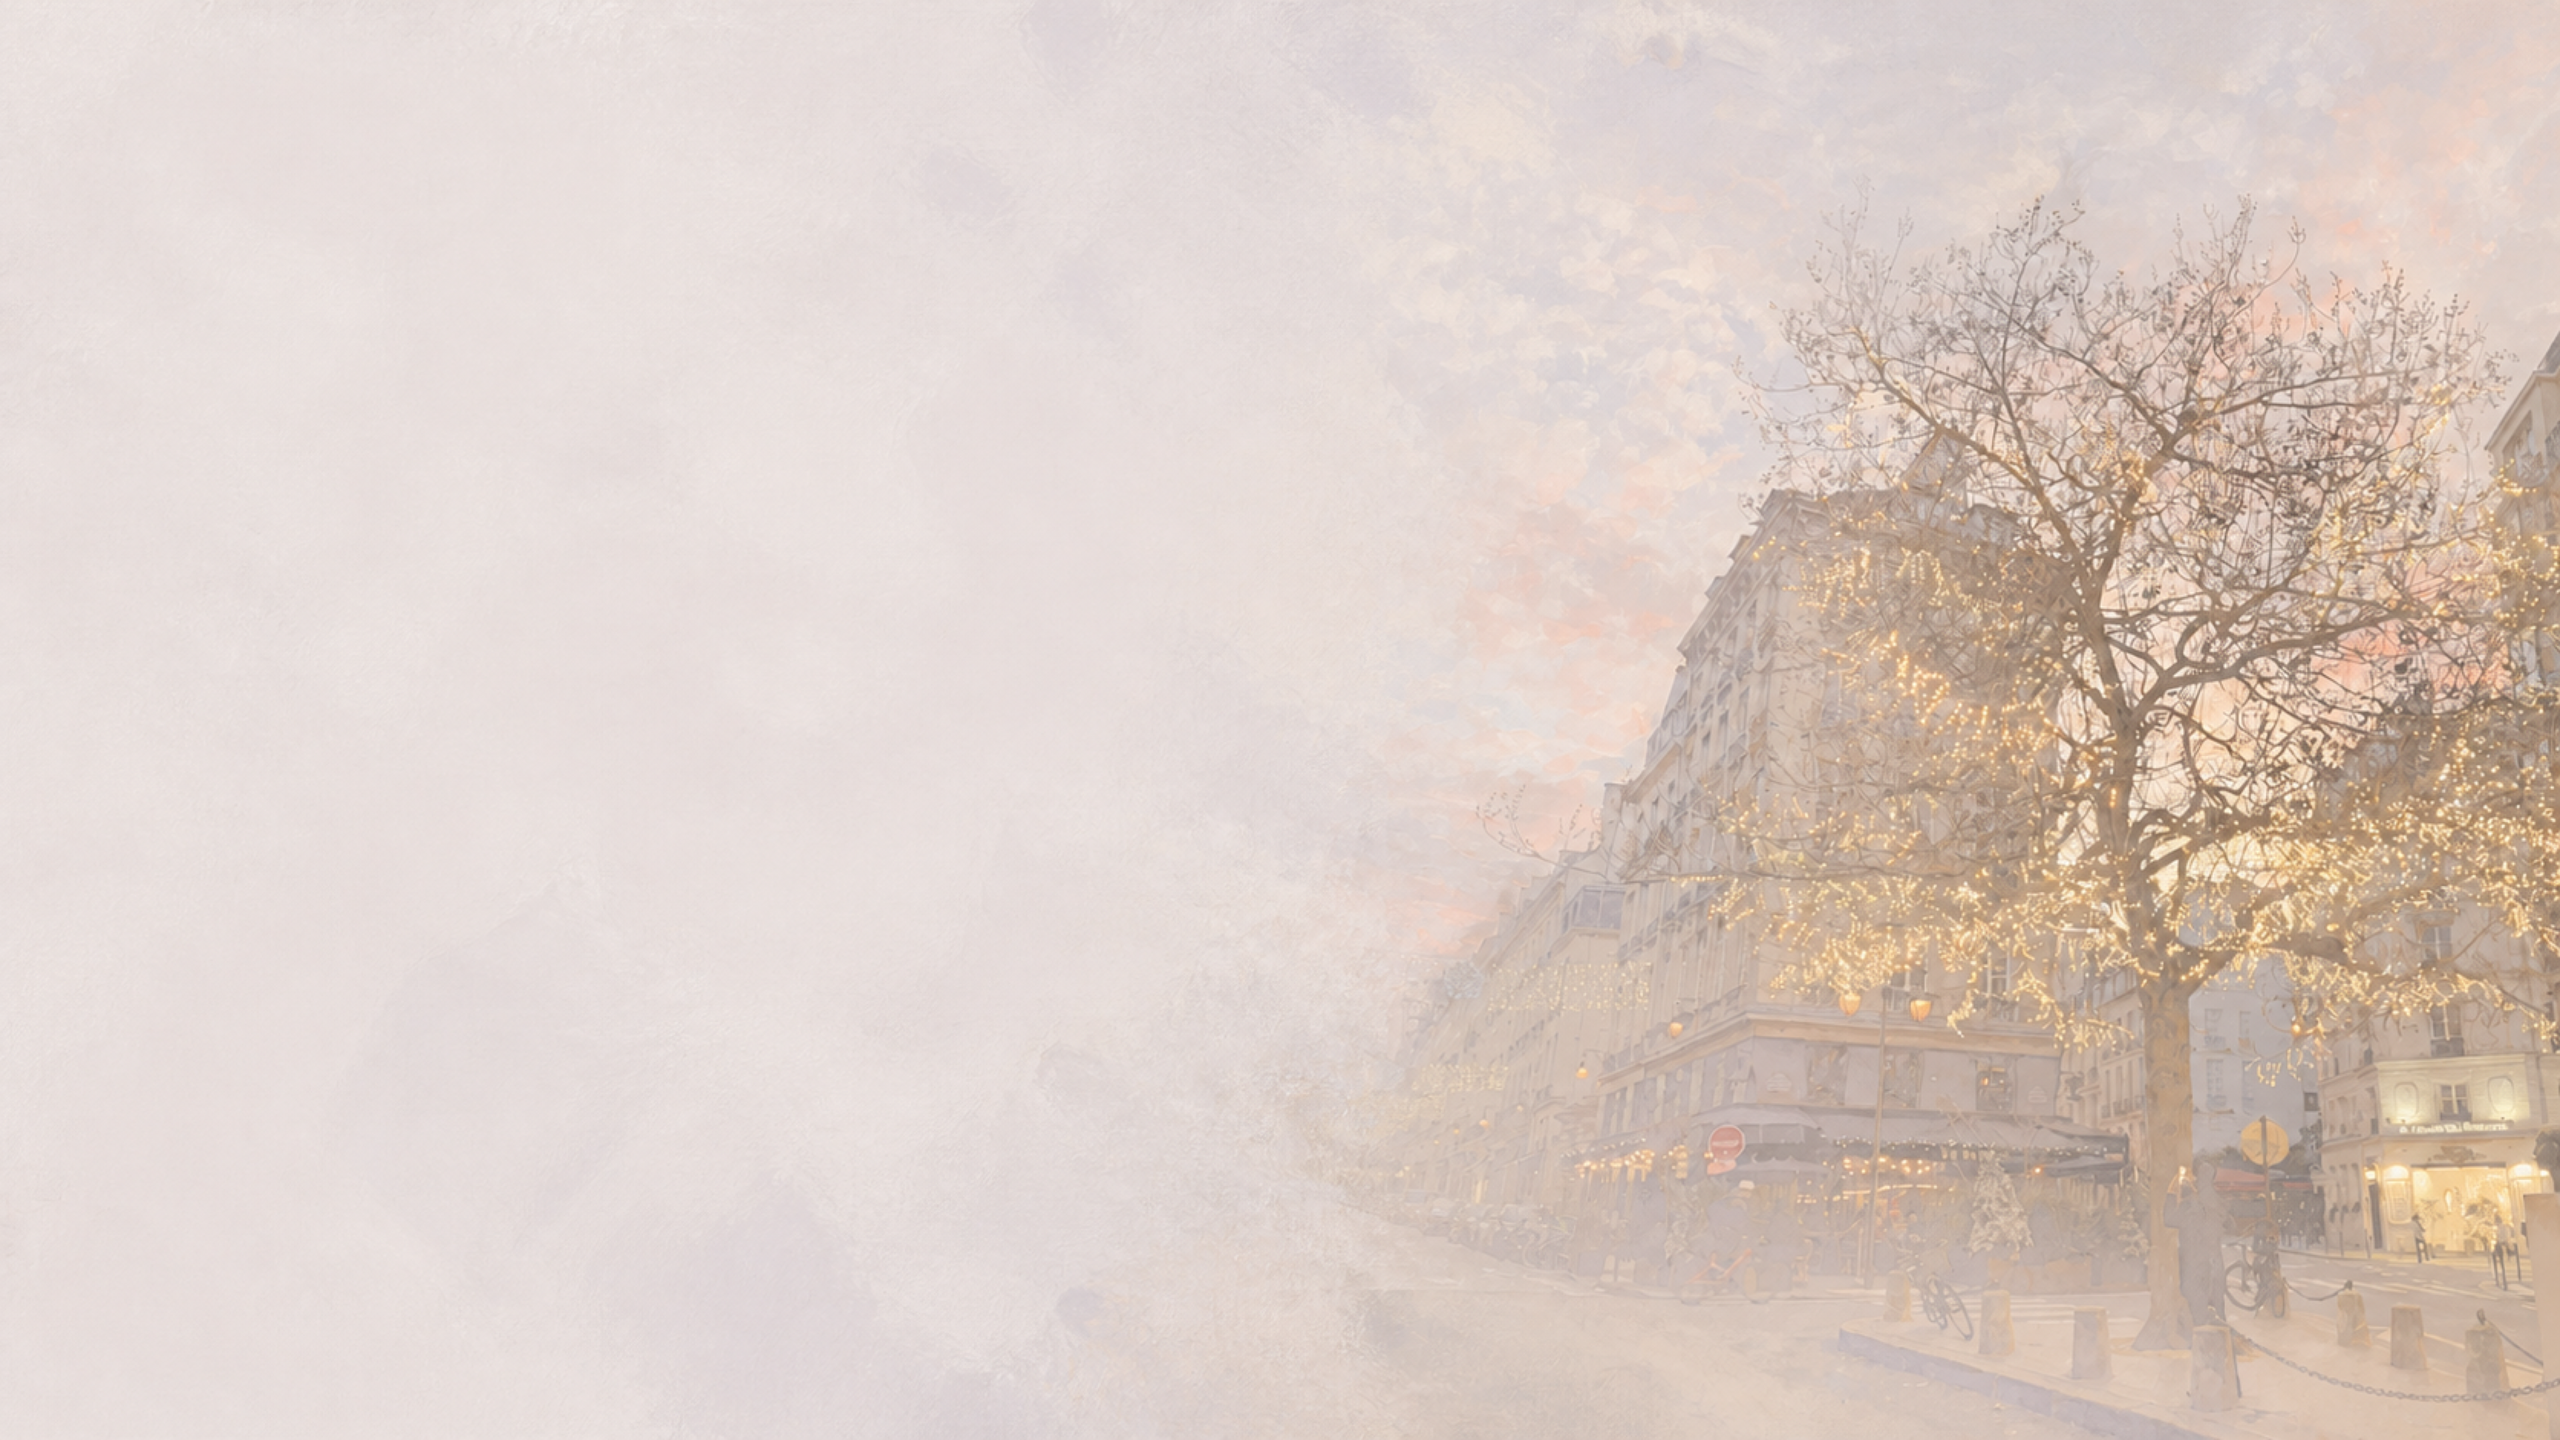
\includegraphics[width = \paperwidth]{figures/cover-oilwash.png}};%
}

% The palette laid out as a swatch card down the right third.
\newcommand{\morandiartBands}{%
  \fill[color5] ([xshift = 0.620\paperwidth]current page.south west) rectangle ([xshift = 0.720\paperwidth]current page.north west);
  \fill[color4] ([xshift = 0.720\paperwidth]current page.south west) rectangle ([xshift = 0.795\paperwidth]current page.north west);
  \fill[color1] ([xshift = 0.795\paperwidth]current page.south west) rectangle ([xshift = 0.905\paperwidth]current page.north west);
  \fill[color3] ([xshift = 0.905\paperwidth]current page.south west) rectangle ([xshift = 0.950\paperwidth]current page.north west);
  \fill[color2] ([xshift = 0.950\paperwidth]current page.south west) rectangle ([xshift = 1.000\paperwidth]current page.north west);%
}
